%%%%%%%%%%%%%%%%%%%%%%%%%%%%%%%%%%%%%%%%%
% APA Assignment Article
% LaTeX Template
% Version 2.0 (February 7, 2023)
%
% This template originates from:
% https://www.LaTeXTemplates.com
%
% Author:
% Vel (vel@latextemplates.com)
%
% License:
% CC BY-NC-SA 4.0 (https://creativecommons.org/licenses/by-nc-sa/4.0/)
%
% NOTE: The bibliography needs to be compiled using the biber engine.
%
%%%%%%%%%%%%%%%%%%%%%%%%%%%%%%%%%%%%%%%%%

%----------------------------------------------------------------------------------------
%	PACKAGES AND OTHER DOCUMENT CONFIGURATIONS
%----------------------------------------------------------------------------------------

\documentclass[
	letterpaper, % Paper size, use either a4paper or letterpaper
	10pt, % Default font size, can also use 11pt or 12pt, although this is not recommended
	unnumberedsections, % Comment to enable section numbering
	twoside, % Two side traditional mode where headers and footers change between odd and even pages, comment this option to make them fixed
]{APAAssignment}

\addbibresource{bibliography.bib} % BibLaTeX bibliography file

\runninghead{MICS CYBER 252, Fall-2024 Hands On Lab Unit 4} % A shortened article title to appear in the running head, leave this command empty for no running head

\footertext{\textit{Hands On Lab Unit 4  } (MICS CYBER 252, Fall -2024)} % Text to appear in the footer, leave this command empty for no footer text

\setcounter{page}{1} % The page number of the first page, set this to a higher number if the article is to be part of an issue or larger work

%----------------------------------------------------------------------------------------
%	TITLE SECTION
%----------------------------------------------------------------------------------------

\usepackage[title,toc,titletoc]{appendix}
\usepackage{titlesec}
\usepackage{lscape}
\usepackage{fontawesome}

\title{Hands On Lab Unit 4 \\ MICS-252, Fall 2024} % Article title, use manual lines breaks (\\) to beautify the layout

% Authors are listed in a comma-separated list with superscript numbers indicating affiliations
% \thanks{} is used for any text that should be placed in a footnote on the first page, such as the corresponding author's email, journal acceptance dates, a copyright/license notice, keywords, etc
% Affiliations are output in the \date{} command
\date{UC Berkleley School of Information \\
MICS Course 252 Fall 2024 (Kristy Westphal)
}


\author{
	Prepared by: Karl-Johan Westhoff \\
	email: \href{mailto:kjwesthoff@berkeley.edu}{kjwesthoff@berkeley.edu}
}


% % Full-width abstract
% \renewcommand{\maketitlehookd}{%
% 	\begin{abstract}
% 		\noindent Lorem ipsum dolor sit amet,rta porttitor.
% 	\end{abstract}
% }

%----------------------------------------------------------------------------------------

\setcounter{tocdepth}{5}
\setcounter{secnumdepth}{5}
\usepackage[title]{appendix}

\begin{document}
\onecolumn
\maketitle % Output the title section

%----------------------------------------------------------------------------------------
%	ARTICLE CONTENTS
%----------------------------------------------------------------------------------------


\section{Log Analysis}\label{log-analysis}

I used the first parts of the ``Six Step Analysis'' we discussed in class, which I have personalized a follows:\footnote{Where each is applied, it is denoted as 'No'*} (when has overkill ever stopped us, the assignment instruction said ``just look at the logs and explain'')
\begin{enumerate}
  \item *Build knowledge, ask around for help (Gather Facts, mobilize help informally and formally) 
  \item *Systematize facts, and communicate (This is where post-it sessions go) 
  \item *Determine biases (Including your own!) 
  \item *Translate Jargon (reference to Richard Feynman\footnote{Richard Feynman was an american theoretical physicist often cited for: “If you can't explain something in simple terms, you don't understand it."\cite{FeynmanMedium} \cite{FeynmanWikipedia}})
  \item *Ensure that test platform works (Calibrate models and remove biases\footnote{Here goes another Feynman Quote: "You must not fool yourself — and you are the easiest person to fool."\cite{FeynmanFoolOurselves}})
  \item *Assure you get the most direct answer (Simplify your reasoning/models as much as possible in your report)
\end{enumerate}


\section{Observations (1*,2*)}\label{observations}

(I mean `Facts', but that word can be charged by opinions and politics,
in an investigation I want absolute objectivity in the beginning, hence the word
`Observations') \\

There are 3 files, two named `log' and one named messages:

\begin{verbatim}
- log file 1.txt
- log file 2.txt
- messages
\end{verbatim}

\subsection{log file 1.txt:}\label{log-file-1.txt}
ASCII text, with CRLF line terminators, 68 lines, each is a log entry (example in Figure \ref{fig:log1} below): \\

\begin{figure}[!htp] % Single column figure
	\centering
	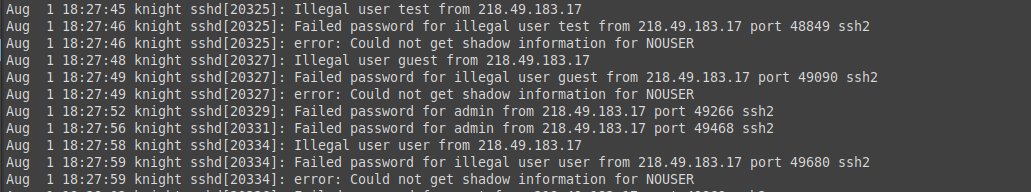
\includegraphics[width=\linewidth]{log1.png}
	\caption{Snippet from "log file 1.txt"}	\label{fig:log1}
\end{figure}

\subsubsection{Log columns/data:} The log entries/data columns are: \\
\texttt{'Month' 'day' 'HH:MM:SS' 'knight' 'sshd[nnnnn]': 'message string'}
\begin{itemize}
  \item The dates are all August 1st, time 18:27:45 to 18:36:28
  \item The \texttt{knight} sting is present in all log entries
  \item The \texttt{sshd{[}number{]}} is related to an OpenSSH server process with the number being the process number on an OpenSSH server 
  \item The \texttt{message} string varies, sometimes containing a username and and ip address/port number.
  \begin{itemize}
	\item The message string can be further subdivided into:\texttt{'Action', 'IP', 'Port'}
	\item The only IP address occurring is "218.49.183.17"
	\item "Failed Password" string occurs in 36 entries
	\item The failed password attempts occur with varying usernames: 'test', 'guest', 'admin', 'root' on varying ephemeral port numbers (rangeing 39604 to 54423)
	\item "error: Could not get shadow information for NOUSER" occurs in 16 entries
  \end{itemize}
\end{itemize}

\subsection{log file 2.txt}\label{log-file-2.txt}
ASCII text, with CRLF line terminators 26 lines, each is a log entry, see snippet in Figure \ref{fig:log2} below: \\
\begin{figure}[!htp] % Single column figure
	\centering
	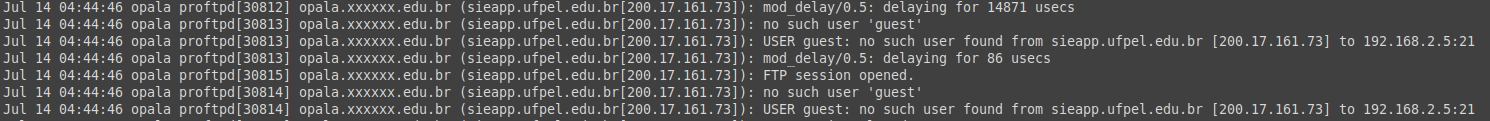
\includegraphics[width=\linewidth]{log2.png}
	\caption{Snippet from "log file 2.txt"}	\label{fig:log2}
\end{figure}

\subsubsection{Log columns/data:} The log entries/data columns are: \\
\texttt{Month day H:MM:SS opala proftpd[nnnnn] opala.xxxxxx.edu.br\ (sieapp.ufpel.edu.br[200.17.161.73]):\ message\ string}
\begin{itemize}
  \item The dates are all July 14th, time 04:44:46 to 04:44:47
  \item The \texttt{opala} sting is present in all log entries.
  \item The \texttt{proftpd[number]} indicates a process on a FTP server from the open source ProFTPD FTP server 
  \item The \texttt{opala.xxxxxx.edu.br\ (sieapp.ufpel.edu.br[200.17.161.73])} is the same for all entries, noting the .edu.br and consistent ip address{[}200.17.161.73{]}
  \item The \texttt{message} string varies, sometimes containing a username and and ip address/port number.
  \begin{itemize}
	\item FTP sessions are opened and closed, 
	\item The username 'guest' is attempted repeatedly for login
	\item The logging time interval is 1s, multiple attempts are done within this short time
	\item mod delay 0.5: delaying for XXX usecs occurs 8 times 
  \end{itemize}
\end{itemize}


\subsection{messages}\label{messages}
Non-ISO extended-ASCII text, with very long lines (1025), with LF, NEL line terminators. 948 lines, each representing an entry \\
Logs entries (example in Figure \ref{fig:messages} below): \\
\begin{figure}[!htp] % Single column figure
	\centering
	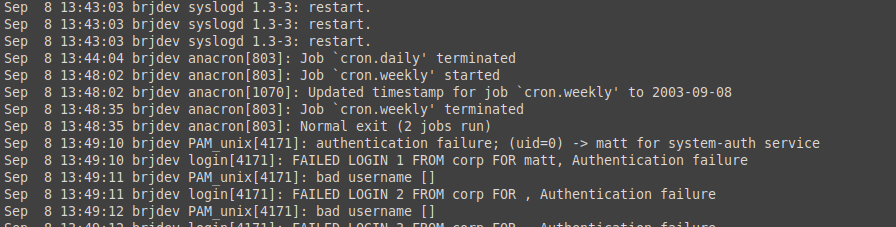
\includegraphics[width=\linewidth]{messages.png}
	\caption{Snippet from "messages"}	\label{fig:messages}
\end{figure}

\subsubsection{Log columns/data:} The log entries/data columns are: \\
\texttt{\textquotesingle{}Month\textquotesingle{}\ \textquotesingle{}day\textquotesingle{}\ \textquotesingle{}HH:MM:SS\textquotesingle{}\ \textquotesingle{}brjdev\textquotesingle{}\ \textquotesingle{}varying\ string\textquotesingle{}:\ \textquotesingle{}message\ string\textquotesingle{}}
\begin{itemize}
   \item The dates are all Sep.8th, time 13:43:03 to 17:20:00
   \item The \texttt{brjdev} string is present in all log entries. 
   \item The \texttt{message} string varies, sometimes containing a username and and ip address/port number.
   \begin{itemize}
	  \item there are log entries from various sources:
	  \begin{itemize}
	      \item syslogd, process doing logging in endpoints (Windows, Mac, Linux)\cite{syslog} in the first log entries this process is restarted 3 times (see Figure\ref{fig:messages})
		  \item anachron, performs periodic command scheduling of processes \cite{anacron}
		  \item CHRON[NNNN], presumably something with chron jobs in Linux/Unix
		  \item pam\_rhosts\_auth, module provides rhost authentication services\cite{pamRhostsAuth}   
		  \item etc.
	  \end{itemize}
	  \item There are some (majority) of very long log entries, with non Ascii characters, starting with: \texttt{Sep  8 HH:MM:SS brjdev SERVER[NNNN]: Dispatch\_input: bad request line}
   \end{itemize}
\end{itemize}


\section{Biases (3*,5*)}
This is a solo assignment so the biases are my own, I have identified the following, which I will need to consider in my analyses:
\begin{itemize}
	\item I suspect there is a some spectacular breach to be identified from these logs, and i want to find it 
	\item This is a course assignment, I think there is a lesson to be learned somewhere
\end{itemize}

\section{Conclusions (6*)}
I have concluded that the files are not related, the logs are from different dates (separated by months) and from different systems, and the IP addresses involved are different in each case. Below are conclusions for each log.



\subsection{log file 1}
\begin{itemize}
  \item OpenSSH is attacked  
  \item Log entries over 8 minutes and 43 seconds, with 68 log entries
  \item Log-in attempts with failed passwords and attempts to retrieve 'shadow information'
  \item different, but generic user names attempted, hereunder 'root' and 'admin'
  \item Attempts from only one ip addess: 218.49.183.17, but from varying remote/ephemeral ports
\end{itemize}

\subsubsection{Hypothesis}
I think this is a brute force attack on an OpenSSH server, SSH gives direct terminal access on the remote host, and high privilege usernames are attempted. The number of attempts and irregular choice of ports and number of attempts on each username suggests a semi manual approach using a script but not a fully automated attack.


\subsection{log file 2}
\begin{itemize}
	\item Many login attempts in short time from IP 200.17.161.73 to FTP server: 192.168.2.5 on port 21, TCP port 21 is the 'control' channel used to negotiate access etc. 
	\item The username ued is 'guest' which sounds generic
	\item FTP sessions are opened and closed many times over 1 second
	\item The server attempts to slow down communication using 'mod\_delay'
\end{itemize}

\subsubsection{Hypothesis}
The log in attempts occur over a short period indicating that it was done automatically, the use of a generic username suggests it may be part of a brute force attack. However, as the log snippet is short, it may also be a part of a DDoS attack and the server does go into mod\_delay 'slowdown mode', what speaks against this is that the attack only comes from one IP. Given the size of the log snippet both brute-force and DDoS are feasible explanations. 

\subsection{messages}
\begin{itemize}
	\item Log entries are from different sources, relating both to internal errors (syslogd is restarted) 
	\item The long SERVER[NNNN] entries, with 'bad request line' could be a log of malformed http requests to a server
\end{itemize}


The messages log seems to be from a SIEM system collecting logs from various places.
The long malformed 'SERVER' messages could indicate and attack on a web server, possibly DDoS or something more fancy on another protocol. I would need some more information (IP addresses, protocols ports etc.) to come up with any conclusions, these can probably be retrieved somehow as the 'messages' file is a log aggregation. \\ 
To better understand the messages, they should be analyzed and sorted by type time etc. I threw the messages (disregarding the long 'SERVER' entries) into ChatGPT, see Appendix Figure \ref{fig:GPT1.png} and Figure \ref{fig:GPT2.png}. Of security interest, the chat GPT 'analysis' revealed: 

\subsubsection{ChatGPT: Authentication Failures} 13:49:10 to 13:49:12: (see Figure \ref{fig:1349}) There are repeated login attempts for matt from a source labeled corp. Authentication fails,  including attempts with a blank username. This could indicate a brute-force or automated script trying to log in to the system, as multiple failed login attempts are recorded in a very short span. \\

\begin{figure}[!htp] % Single column figure
	\centering
	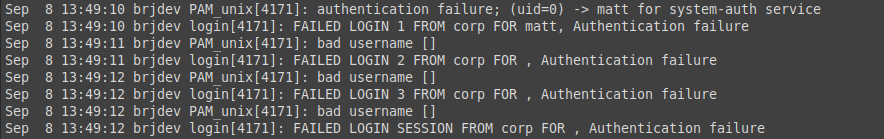
\includegraphics[width=\linewidth]{1349.png}
	\caption{13:49:10 to 13:49:12}	\label{fig:1349}
\end{figure}



\subsubsection{Hypothesis}
Looking at the 'raw' logs, I am not so sure about this, it is 'only' 3 attempts and could be someone misspelling username etc. 3 attempts in 2 seconds I assume that to be humanly possible.

\subsubsection{ChatGPT: Failed Remote Shell (RSH) Attempts} 14:55:41 to 14:59:22:(see Figure \ref{fig:1455}) Several attempts to use the rsh service are made from root@94.90.84.93 as user lpd. All these are denied due to "access not allowed." These multiple attempts indicate an attempt to exploit weak authentication methods like rsh, which is less secure than SSH. \\

\begin{figure}[!htp] % Single column figure
	\centering
	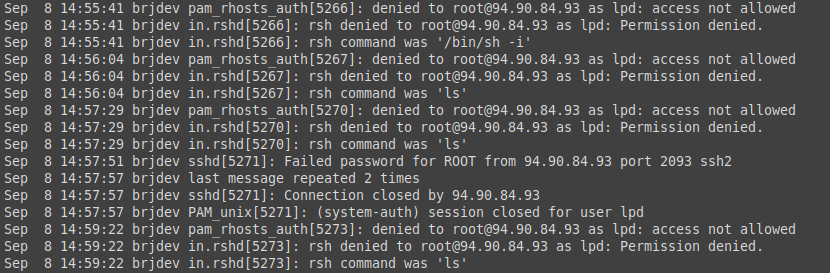
\includegraphics[width=\linewidth]{1455.png}
	\caption{14:55:41 to 14:59:22}	\label{fig:1455}
\end{figure}

\subsubsection{Hypothesis}
There are 5 attempts over 2 minutes, this could be someone poking around with rsh, or an administrator forgetting a password, would need to check up on who 94.90.84.93 is.  

This log analysis has identified items for further investigation.


%----------------------------------------------------------------------------------------
%	 REFERENCES
%----------------------------------------------------------------------------------------
\clearpage
\printbibliography % Output the bibliography

%----------------------------------------------------------------------------------------



%----------------------------------------------------------------------------------------
%	 Appendices
%----------------------------------------------------------------------------------------

\appendix


\clearpage
\chapter{Appendices}
\begin{appendices}
\begin{figure}[!htp] % Single column figure
	\centering
	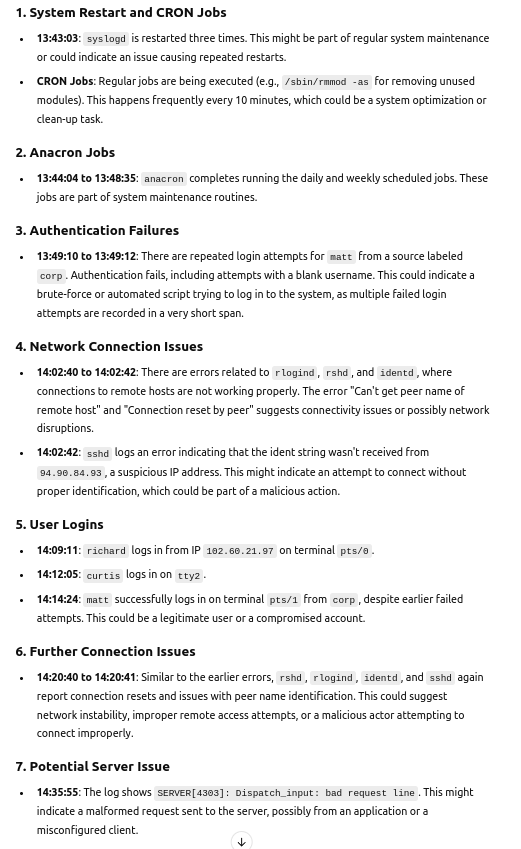
\includegraphics[width=0.7\linewidth]{GPT1.png}
	\caption{ChatGPT analysis of logs before the large chunk of 'SERVER' logs}	\label{fig:GPT1.png}
\end{figure}
\begin{figure}[!htp] % Single column figure
	\centering
	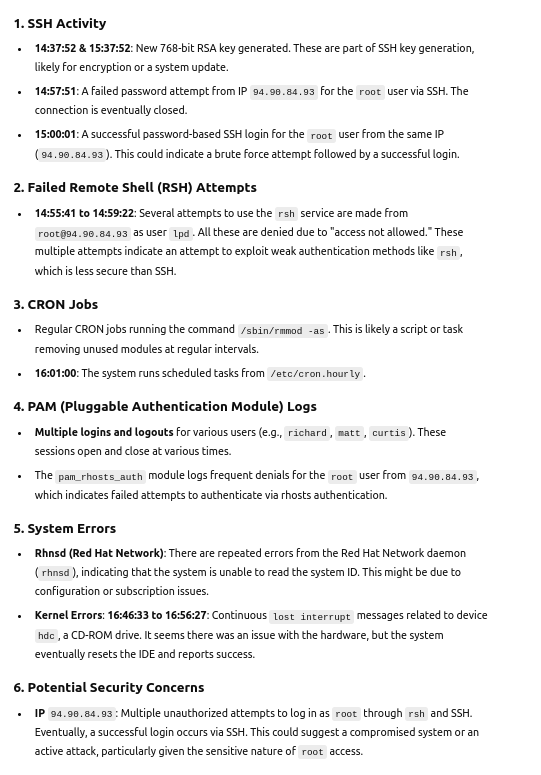
\includegraphics[width=0.7\linewidth]{GPT2.png}
	\caption{ChatGPT analysis of logs after the large chunk of 'SERVER' logs}	\label{fig:GPT2.png}
\end{figure}



\end{appendices}
\end{document}
